%%%%%%%%%%%%%%%%%%%%%%%%%%%%%%%%%%%%%%%%%
% Short Sectioned Assignment
% LaTeX Template
% Version 1.0 (5/5/12)
%
% This template has been downloaded from:
% http://www.LaTeXTemplates.com
%
% Original author:
% Frits Wenneker (http://www.howtotex.com)
%
% License:
% CC BY-NC-SA 3.0 (http://creativecommons.org/licenses/by-nc-sa/3.0/)
%
%%%%%%%%%%%%%%%%%%%%%%%%%%%%%%%%%%%%%%%%%

%----------------------------------------------------------------------------------------
%	PACKAGES AND OTHER DOCUMENT CONFIGURATIONS
%----------------------------------------------------------------------------------------

\documentclass[paper=a4, fontsize=11pt]{scrartcl} % A4 paper and 11pt font size

\usepackage[T1]{fontenc} % Use 8-bit encoding that has 256 glyphs
\usepackage{fourier} % Use the Adobe Utopia font for the document - comment this line to return to the LaTeX default
\usepackage[english]{babel} % English language/hyphenation
\usepackage{amsmath,amsfonts,amsthm} % Math packages

\usepackage{lipsum} % Used for inserting dummy 'Lorem ipsum' text into the template

\usepackage{sectsty} % Allows customizing section commands

\usepackage{graphicx}
\usepackage{todonotes}

\allsectionsfont{\centering \normalfont\scshape} % Make all sections centered, the default font and small caps

\usepackage{fancyhdr} % Custom headers and footers
\pagestyle{fancyplain} % Makes all pages in the document conform to the custom headers and footers
\fancyhead{} % No page header - if you want one, create it in the same way as the footers below
\fancyfoot[L]{} % Empty left footer
\fancyfoot[C]{} % Empty center footer
\fancyfoot[R]{\thepage} % Page numbering for right footer
\renewcommand{\headrulewidth}{0pt} % Remove header underlines
\renewcommand{\footrulewidth}{0pt} % Remove footer underlines
\setlength{\headheight}{13.6pt} % Customize the height of the header

\numberwithin{equation}{section} % Number equations within sections (i.e. 1.1, 1.2, 2.1, 2.2 instead of 1, 2, 3, 4)
\numberwithin{figure}{section} % Number figures within sections (i.e. 1.1, 1.2, 2.1, 2.2 instead of 1, 2, 3, 4)
\numberwithin{table}{section} % Number tables within sections (i.e. 1.1, 1.2, 2.1, 2.2 instead of 1, 2, 3, 4)

\setlength\parindent{0pt} % Removes all indentation from paragraphs - comment this line for an assignment with lots of text

%----------------------------------------------------------------------------------------
%	TITLE SECTION
%----------------------------------------------------------------------------------------

\newcommand{\horrule}[1]{\rule{\linewidth}{#1}} % Create horizontal rule command with 1 argument of height

\title{	
\normalfont \normalsize 
\textsc{Vienna University of Technology} \\ [25pt] % Your university, school and/or department name(s)
\horrule{0.5pt} \\[0.4cm] % Thin top horizontal rule
\huge Demonstration of K-Nearest-Neighbor \\ % The assignment title
\horrule{2pt} \\[0.5cm] % Thick bottom horizontal rule
}

\author{Benjamin Kiesl \and Philipp Steinwender \and Robert Sch\"{a}fer} % Your name

\date{\normalsize\today} % Today's date or a custom date

\begin{document}

\maketitle % Print the title

%----------------------------------------------------------------------------------------
%	PROBLEM 1
%----------------------------------------------------------------------------------------

\section{Our Task}

You should pick a number of 2D (or optionally 3D) datasets (where the variables correspond to the coordinates in the 2D or 3D space), and demonstrate how different settings of the parameter k in K-NN modify the decision boundary. Your solution should work with arbitrary number of classes.
Provide an interface that visualises the data set and its classes. In that interface, provide controls where the user can select a k value, and colour the points in the space according to which class they would get classified into. A simple approach is to iterate over all your points in the visualisation grid and ask the classifier for the classification of each point.

Finally, provide an option to the user to select a training/test set split, and indicate the classification of the test set in your plot.
The data sets you provide should contain examples where low numbers of k are superior, as well as examples where higher number of k are more accurate.

\section{Implementation}

For this assignment we have two implementations: one in Java and a second one in R.

\subsection{kNN visualization in Java}

To visualize the decision boundaries and  classification results of weka's kNN implementation iBK a Java gui was implemented. We used Swing and plain Java. There is also a dataset generator for multiple gaussian cluster that can only be executed after editing the code and recompilation of the application.

To run the application, execute the \texttt{knn-java-gui/run.sh} script. There is also a script to compile the source \texttt{knn-java-gui/compile.sh}. Both scripts also have versions for windows.

\begin{figure}[\textwidth]
    \begin{center}
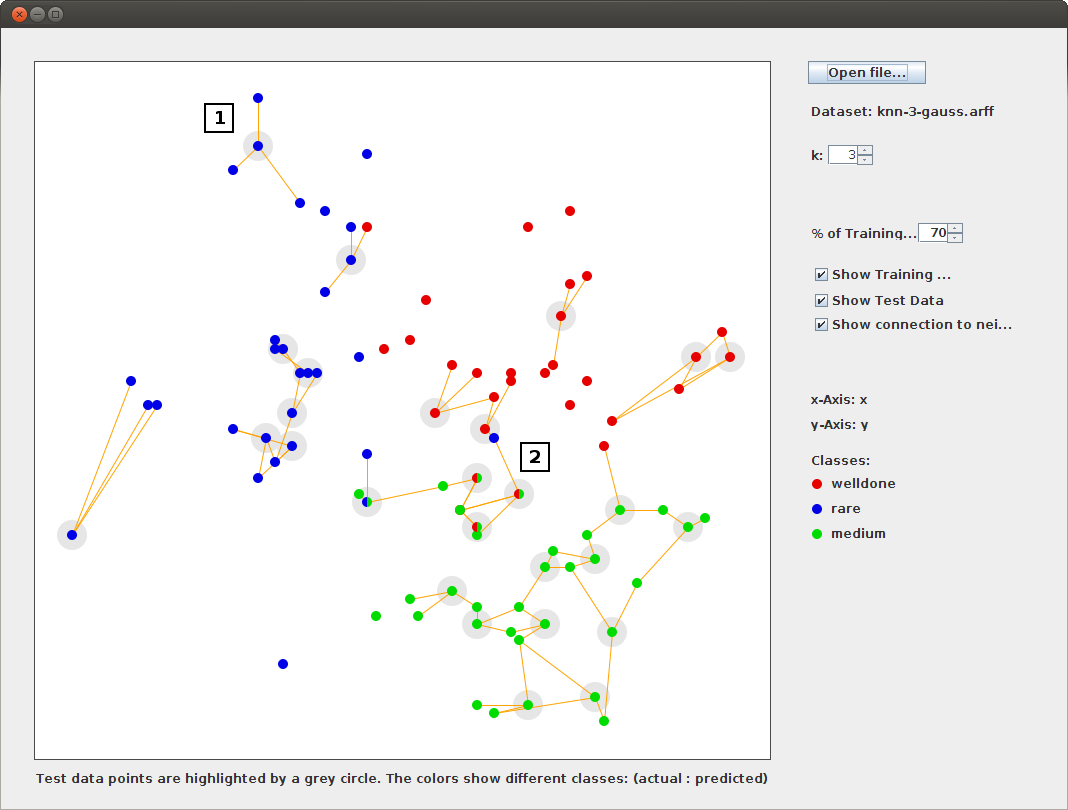
\includegraphics[width=\textwidth]{knn-visualization-marker}
    \end{center}
\caption{Java GUI}
\label{fig:javagui}
\end{figure}

Figure \ref{fig:javagui} shows how the gui looks like and which controls there are for manipulating the parameters of the data set and the classifier. The drawing area on the left displays the data points on a two dimensional coordinate system. The coordinate values of the data set get scaled to fit this area. The two markers showing the numbers 1 and 2 were added after taking the screenshot and highlight the following features:

\begin{enumerate}
\item With these 4 blue data points can be described how we visualize the decision boundaries of knn. The blue point in the middle has a light grey bigger circle around it. Points that look like this are from the test set. Data point that do not have this light grey highlighting are data points from the training set. Each data point of the test set has \texttt{k} connectors to surrounding data points which are the k nearest neighbors of the point.
\item Here we can see a half red half green data point of the test set. It is connected with 2 green data points and a blue one. Therefore the classifier predicts its class as green. The predicted class can be seen in the right half of the data point. The left half shows which class the data point acutally has which is red. If theclassifier predicts the true value of a data point, both halfs have the same color.
\end{enumerate}

On the right side of the gui is a control panel. From top to bottom:

\begin{itemize}
\item The "open file" button can be used to read an arff file from disk. After selecting a file, it's content is loaded, a classifier is created and the result gets drawn. Below is a label that displays the name of the currently selected file.
\item The spinner with the label \texttt{k} can be used to modify the classifier's value of \texttt{k}.
\item The training-test-split can be modified with the spinner showing the number 70 whereby this means that we do a 70\% split and use 70\% for training and the rest for classification. Although kNN does not train a model, this parameter tells the classifier how much unclassified instances it should use.
\item The next three checkboxes can be used to view or hide specific visualization details. One can hide the data points of the training data, those of the test set and hide the connectors between the test data points and their nearest neighbors.
\item Then there is a legend telling the attribute names and which coloreach class is assigned to.
\end{itemize}

All controls have a ChangeListener that redraws the data points and the results immediately after a value got changed by the user.

When loading a new file, the data is read by weka's arff parser. The created \texttt{Instances} are split by the specified percentage using the \texttt{RemovePercentageFilter}. Before the spilt, the data is shuffled. Then the \texttt{iBK} classifier gets instantiated, configured and the data points are drawn.

With this visualization one can easily recognize how the classifier predicts the class of a new instance and how the values of k and the train-test-set-split can change runtime behaviour.




\subsection{kNN visualization in R}

We used R as a wrapper for Weka and plotted the result with the native functionality in R. Our R-Script can handle 2- and 3-dimensional data as well as separate test and training data. It visualizes either the predicted instances of the test data itself or visualizes how many of them were classified correctly. After plotting the results, the user is asked to specify another k-parameter and the script runs the visualization once again with the new parameter.

\subsubsection{Evaluation}
Our Data Sets were 
\begin{enumerate}
\item
    The 'Skin-NonSkin' Data Set, which is a collection of RGB-values and the 4th attribute states whether this is a skin color or not
\item
    A truncation of the iris data set, where we have removed the 4th column to adjust the data to three dimensions.
\item
    The 'Haberman's Survival' data set, which contains cases from a study on the survival of patients who had undergone surgery for breast cancer.
\end{enumerate}

The K-NN nearest neighbor performs especially well if we have a balanced data set with separated spaces where one of the class values is dominating. Figure \ref{fig:skin:predicted:k5} shows the prediction of K-NN for the 'Skin-Nonskin' data set. Obviously, there is a certain space where all the actual skin colors are located. This is an important fact, which facilitates the prediction of instances. In figure \ref{fig:skin:correct:k5} one can see the same data set visualized based on the correctness of the prediction. Black marks belong to correct instances and white marks belong to misclassified instances. In this example, K-NN performs very well, only few instances located on the boundary between the two spaces are misclassified.

\begin{figure}[0.5\textwidth]
    \begin{center}
        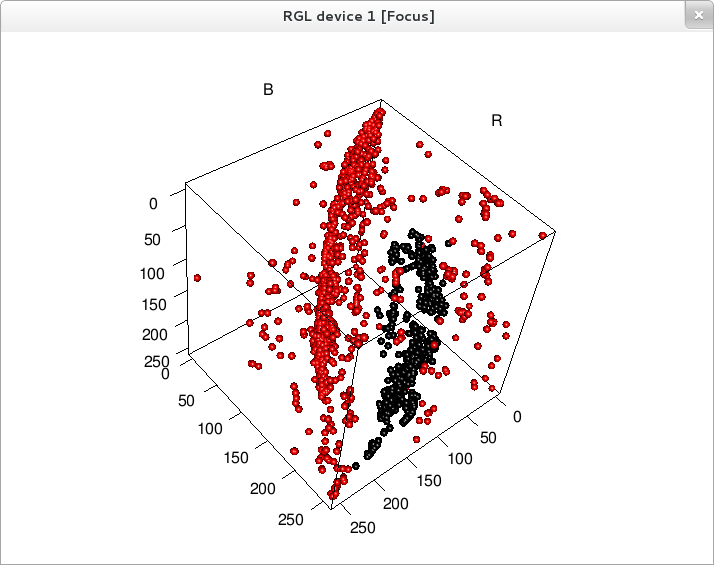
\includegraphics[width=0.5\textwidth]{Skin_predicted_k5}
    \end{center}
    \caption['Skin-NonSkin' prediction with k=5]{The 'Skin-NonSkin' Data Set, colored by the predicted class attribute, with 5 neighbors as K parameter.}
    \label{fig:skin:predicted:k5}
\end{figure}

\begin{figure}[0.5\textwidth]
    \begin{center}
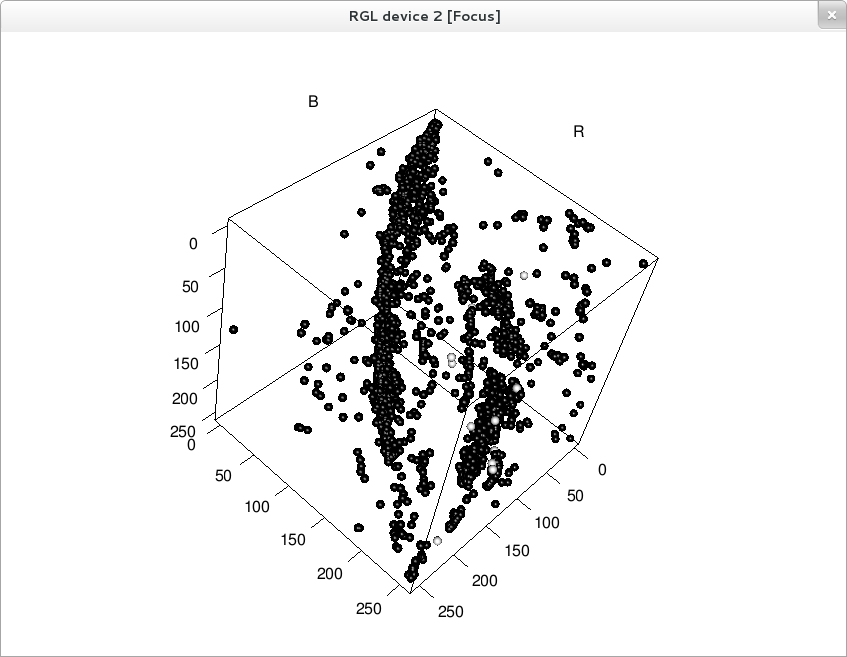
\includegraphics[width=0.5\textwidth]{Skin_correct_k5}
    \end{center}
\caption['Skin-NonSkin' correctness with k=5]{The 'Skin-NonSkin' Data Set, colored by correct or misclassified instance, with 5 neighbors as K parameter.}
\label{fig:skin:correct:k5}
\end{figure}

If we raise the K-parameter up to 100, we get worse results. As seen in figure \ref{fig:skin:predicted:k100} the K-NN algorithm misclassfies a couple of instances that are located in one corner of the RGB space. Hence, we can see more white marks in figure \ref{fig:skin:correct:k100}.

\begin{figure}[0.5\textwidth]
    \begin{center}
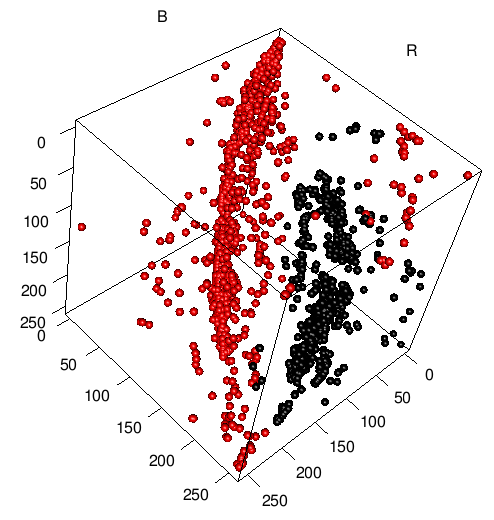
\includegraphics[width=0.5\textwidth]{Skin_predicted_k100}
    \end{center}
\caption['Skin-NonSkin' prediction with k=100]{The 'Skin-NonSkin' Data Set, colored by the predicted class attribute, with 100 neighbors as K parameter.}
\label{fig:skin:predicted:k100}
\end{figure}


\begin{figure}[0.5\textwidth]
    \begin{center}
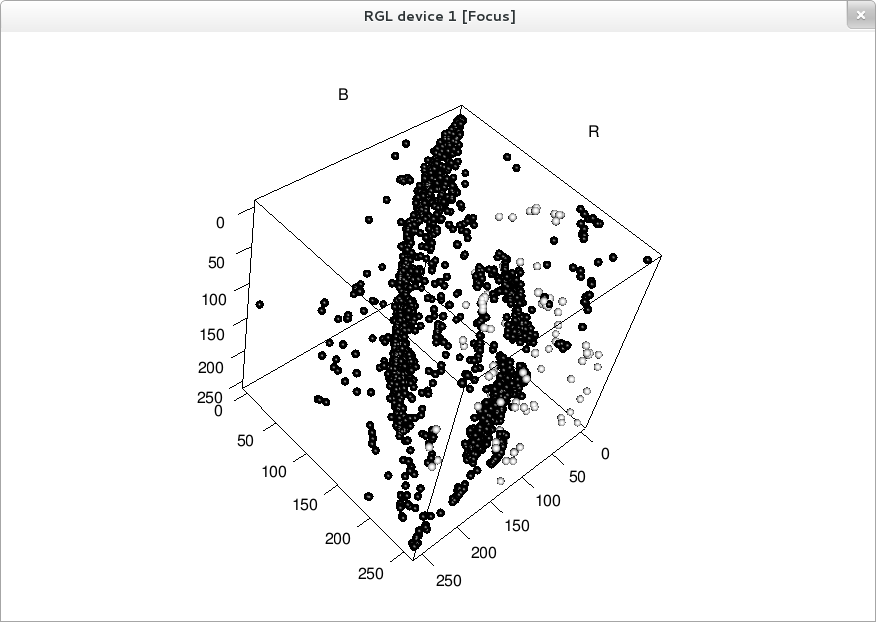
\includegraphics[width=0.5\textwidth]{Skin_correct_k100}
    \end{center}
\caption['Skin-NonSkin' correctness with k=100]{The 'Skin-NonSkin' Data Set, colored by correct or misclassified instance, with 100 neighbors as K parameter.}
\label{fig:skin:correct:k100}
\end{figure}

We observe a similar result for the truncated 'Iris' data set. K-NN works very well except for some instances on the boundaries, figure \ref{fig:iris:correct:k5} shows us misclassfied instances exactly on the hyperplane between 'Iris versicolor' and 'Iris virginica'. The predicted instances can be seen in figure \ref{fig:iris:predicted:k5}.
\begin{figure}[0.5\textwidth]
    \begin{center}
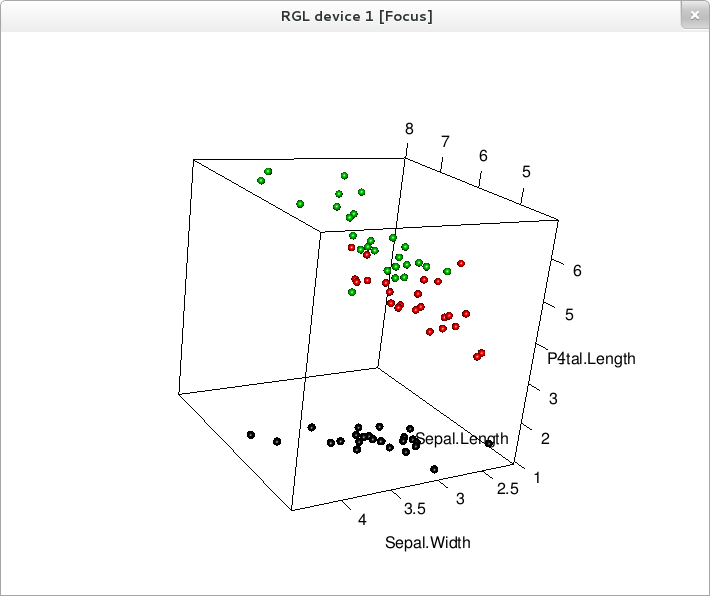
\includegraphics[width=0.5\textwidth]{Iris_predicted_k5}
    \end{center}
\caption['Iris' prediction with k=5]{The 'Iris' Data Set, colored by the predicted class attribute, with 5 neighbors as K parameter.}
\label{fig:iris:predicted:k5}
\end{figure}


\begin{figure}[0.5\textwidth]
    \begin{center}
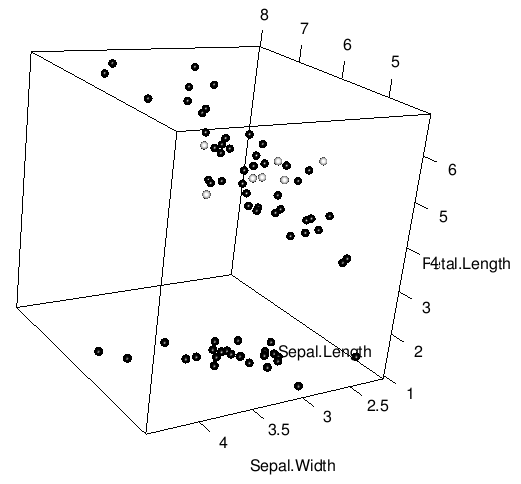
\includegraphics[width=0.5\textwidth]{Iris_correct_k5}
    \end{center}
\caption['Iris' correctness with k=5]{The 'Iris' Data Set, colored by correct or misclassified instance, with 5 neighbors as K parameter.}
\label{fig:iris:correct:k5}
\end{figure}

Unlike the two previous data sets, the 'Haberman' data set does not contain clearly separable spaces where one of the class values dominates. Accordingly, the K-NN algorithm performs rather poor on this input set. Figure \ref{fig:haberman:correct:k13} shows the best distribution of correct and misclassified instances, namely 31 misclassified and 131 correctly classfied instances. It is notably that a k parameter of 13 is a rather high value. This fact could be interpreted in a sense that low k-values are preferable in case of easily separable data sets and higher k-values should be used for more overlapping, more scattered data sets.
\begin{figure}[0.5\textwidth]
    \begin{center}
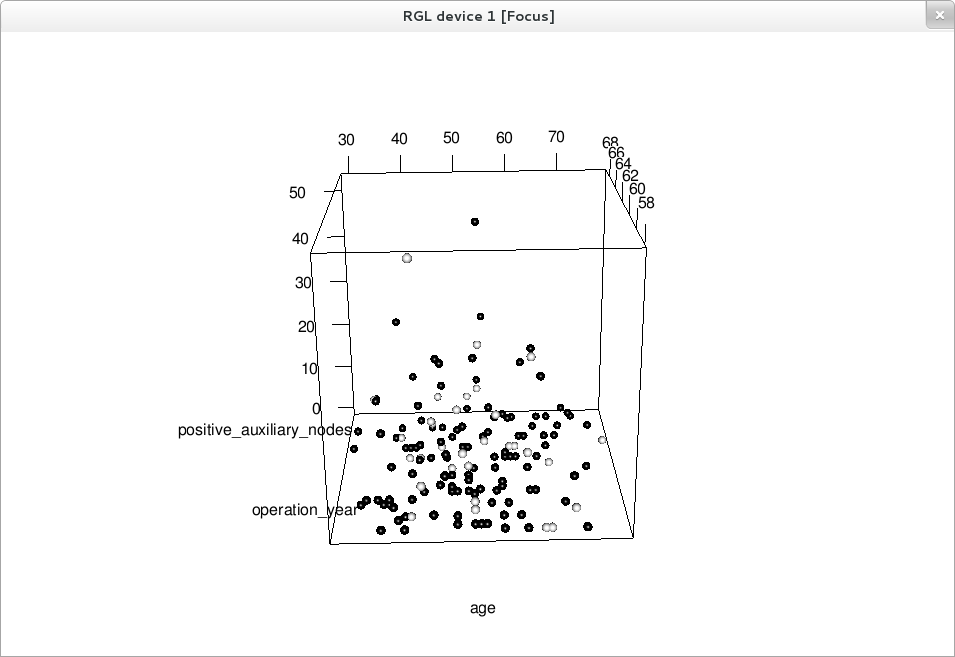
\includegraphics[width=0.5\textwidth]{Haberman_correct_k13}
    \end{center}
\caption['Haberman' correctness with k=13]{The 'Haberman' Data Set, colored by correct or misclassified instance, with 13 neighbors as K parameter.}
\label{fig:haberman:correct:k13}
\end{figure}
\end{document}
